\documentclass[a4paper,10pt,twocolumn,twoside]{article} %Pour une colonne il vous suffit de retirer "twocolumn,"
\usepackage{tpl3}
\usepackage{lipsum}
\usepackage{amsmath}
\usepackage{hyperref}

%Pour mettre les vecteurs en gras, il faut dé commenter la ligne suivante 
%\renewcommand{\vec}[1]{\boldsymbol{\mathbf{#1}}} 

%-----------------------------Début du document---------------------------------
\begin{document}

\twocolumn[{%
\begin{@twocolumnfalse}
\logo
\marginmark
\header{Économétrie II}{Master 2 EEET}\\     % Matière et n° du TP

\begin{flushright}
\titre{{\strut \huge \bfseries \sffamily  \hspace*{7 cm}Évolution de la demande en électricité à l'horizon 2030}}\\ [0.15cm]                              % Titre du TP
\end{flushright}
% \vspace{-0.3cm}
\auteur{{\strut\hfill\Large \sffamily {Thomas Da Costa$^{1, 3}$, Léa Guillaut$^{2, 3}$}}}\\[0.1cm]                                      %Auteur du TP
\vspace*{-0.01cm}
\formation{{\strut\hfill  \sffamily $^1$École Normale Supérieure -- Université Paris Sciences et Lettres (ENS - PSL)}  }  \\[0.cm]     
\formation{{\strut\hfill  \sffamily $^2$Institut d'Études Politiques de Paris (SciencePo Paris)}}  \\[0cm]
\formation{{\strut\hfill  \sffamily $^3$AgroParisTech -- Université Paris-Saclay}  }  \\[0.cm]   %Formation/Option
\vspace*{-0.45cm}

{\color{color2}\rule{\textwidth}{.8pt}}\vspace{0.1cm}
\resume{%le résume

À faire : 
\begin{itemize}
\item Pour des time-series seules : univariate analysis.
    \begin{itemize}
        \item \textbf{Tester quelles variables sont stationnaires autour d'une trend déterministe} $\to$ ça nous permet de savoir ensuite si on peut faire des ARIMA, etc. Plot Autocorrelogram by using (partial) autocorrelation function. If the PACF of residuals is out of the confidence interval for a given lag $k$, the process has to be respecified as regards the choice of $p$ or $q$. Ljung-Box + Shapiro Wilk over residuals.
        \item unit root: determine whether a time series variable is non-stationary and possesses a unit root, meaning it exhibits a stochastic trend. If a time series has a unit root, it implies that the series follows a random walk and that shocks to the system have permanent effects, making it non-mean reverting. \textbf{Elliott-Rothenberg-Stock (ERS) Test and KPSS Test}.
    \end{itemize}
\item Multivariate time series = dynamical modelization of a vector of
time series. 
\begin{itemize}
    \item BIC over ARDL model to choose variables and lags.
    \item If non-stationary, go in log then first difference (approximation of the growth rate). If non-stationary, OLS is inconsistent.
    \item Reproduire QM1-PS5 en controlant la consommation d'électricité par la taille de la population et en retirant IRC. On choque l'indice des prix à la consommation. Short-run restriction (ordered data) with 10 lags.
    \item Structural VAR: ordering of the endogenous variables from the most
    exogeneous: IPC > Prix de l'électricité > Consommation d'électricité (corrigée de la taille de la population) > PIB.
    \item Si structural VAR, GIRF et choc sur le prix de l'électricité // choc sur l'inflation.
    \item \textbf{Vector AutoRegression} $\to$ Impulse Response Function, construire des chocs sur le prix de l'électricité $\to$ voir ce qu'il se passe sur la consommation. See E2-PC4.
    \item Regarder les codes R du chap 2 \href{https://www.dropbox.com/scl/fo/5wj88417eeloxca22qk0b/ACA2WKJ9yp2t9NGVqWXIiks?dl=0&e=1&rlkey=yjyfxpotil48wx9hh4xkdiq68}{ici}.
    \item Dire que notre SVAR souffre d'un omitted variable bias en n'ayant pas pris en compte l'IRC. Interesting to add a Markov Switching process to account for IRC (up or down). Or use an Error Correction Model if our variables are non-stationary (Co-integrated VAR).
\end{itemize}
\item Utiliser le package ts pour gérer les time series.
\item Account for structural break in 2020? see E2-PC1.
\item \textbf{Shapiro-Wilk test} for normality of residuals (small samples). Jarque-Bera test is better for large samples. 
\item On peut se contenter d'interpréter le tableau de régression tout prêt.
\item Investiguer la méthode LASSO ou RIDGE pour sélectionner les variables. 
\item Utiliser des BIC plutôt que AIC pour sélectionner les variables.
\item Transformer IPC en taux d'inflation: $\pi = 100 \cdot \frac{IPC_t - IPC_{t-1}}{IPC_{t-1}}$ ?
\item Prévision 2030: si on utilise des AR process, on peut aisément faire des prévisions par régressions successives.
\item Intéressant d'avoir $log(c_{elec})_t = \alpha + \boldsymbol{\beta X_t} + \boldsymbol{\gamma X_{t-1}} + {\chi log(c_{elec})_{t-1}} + \varepsilon$? $\to$ Breusch–Godfrey test for autocorrelation (The regression models to which the test can be applied include cases where lagged values of the dependent variables are used as independent variables in the model's representation for later observations. BG test requires the assumptions of stronger forms of predeterminedness and conditional homoscedasticity.). If excluding $\chi log(c_{elec})_{t-1}$, the Ljung-Box test can be used (valid assumption of strict exogeneity).
\end{itemize}

}\vspace{0.1cm}            % Voir le fichier "resume.tex"
\keywords{\rm Économétrie, Régression Linéaire, Prédiction.}\vspace{0.15cm} \\           % Mots clefs
\end{@twocolumnfalse}}]

%----------------------------Headers et Footers---------------------------------

\pagestyle{fancy}
\fancyhf{}

\newcommand{\headere}{Master 2 EEET}            % Header externe
\newcommand{\headeri}{Econométrie II}              % Header interne
\newcommand{\footeri}{AgroParisTech}   % Footer interne

\thispagestyle{plain}
\headers

%----------------------------------Contenu--------------------------------------

\section{Notes en vrac}

\subsection{Notes cours C. Doz}

\subsubsection{Univariate time series}
Stationary around a deterministic trend: $X_t = a + bt + Y_t$ where $(Y_t)_t \in Z$ is a stationary process. (Stationarity if esperance and variance does not depend on $t$).

White noise: variance is constant, no autocorrelation, mean is zero.

Wold theorem: any stationary process can be written as a linear combination of white noise. $X_t = m + \sum_{i=0}^{\infty} \psi_i \varepsilon_{t-i}$. \\


Lag operator: $LX_t = X_{t-1}$. Now, if $(X_t)_t$ is a stationary process:
\begin{itemize}
    \item $AR(p)$ process: $X_t = \mu + \sum_{i=1}^{p} \phi_i X_{t-i} + \varepsilon_t$.
    \item Best Linear Forecast of an $AR(p)$ process: $X^*_{t+1\vert t} = \mu + \sum_{i=1}^{p} \phi_i X_{t+1-i} + \varepsilon_t$.
    \item Moving average process $MA(q)$: $X_t = \mu + \varepsilon_t + \sum_{i=1}^{q} \theta_i \varepsilon_{t-i}$.
    \item $ARMA(p, q)$ process: $X_t = \mu + \sum_{i=1}^{p} \phi_i X_{t-i} + \varepsilon_t + \sum_{j=1}^{q} \theta_j \varepsilon_{t-j}$.
    \item \textbf{If $(X_t)_t$ is an $ARMA(p, q)$ process, autocorrelation should tend exponentially to 0 with increasing lags.}
    \item On these processes, the impact of a shock is transitory.
\end{itemize}

\textit{In our case, electricity consumption might not be ARMA processes, so we might not be able to forecast as such... it is to be tested. We have to test which variables can be considered stationary around a deterministic trend.}

Now, if $X_t = \mu + X_{t-1} + \varepsilon_t$ (random walk), we have: 
\begin{itemize}
    \item ARIMA: $(1 - L)^d \Phi(L)X_t = \mu + \theta(L) \varepsilon$
    \item On ARIMA process, the impact of a shock is permanent.
    \item Autocorrelation of $X_t$ don't exponentially tend to 0 with increasing lags.
    \item Identication and estimation of an $ARIMA(p,d,q)$ :
    \begin{enumerate}
    \item choice of d : visual inspection of the estimated
    autocorrelogram + unit root tests (see below).
    \item If $(X_t)_t$ appears to be non-stationary, study $(1-L)X_t$, etc...
    \item Choose the smallest $d$ such that $(1-L)^d X_t$ appears to be stationary.
    \item choice of (p,q) : compute $Y_t = (1-L)^d X_t$ and apply to $Y_t$ the procedure which has been presented for ARMA(p,q).
    Estimate an ARMA model for $Y_t$.
    \end{enumerate}
\end{itemize}

\subsubsection{Multivariate time series}
Let's consider a vector of time series $(X_t)_t$ with $X_t = (X_{1t}, X_{2t}, \ldots, X_{kt})$. We suppose that $(X_t)_t$ is a stationary process. 

Wold theorem: 
If $(X_t)_t$ is a stationary process and $(\varepsilon_t)_t$ is a white noise, then $(X_t)_t$ can be written as a linear combination of $(\varepsilon_t)_t$: $$X_t = m + \sum_{i=0}^{\infty} A_i \varepsilon_{t-i}, \quad A_0 = I, \sum_{i = 1}^\infty A_i < \infty$$ \\

VAR(p): $X_t = \mu + \sum_{i=1}^{p} \Phi_i X_{t-i} + \varepsilon_t \Leftrightarrow  \Phi(L)X_t = \mu + \varepsilon_t$. \\

\textit{It's not clear that IRC is a good variable to include in the VAR model: it does not seem to be an AR(1) process, or at least not with our granularity.}

To do an IRF: Cholesky decomposition to have an orthogonalized impulse response function.

\subsection{Notes Ferrara - Doz}
\begin{enumerate}
    \item Data analysis
    \item Model specification
    \item Parameter estimation
    \item Model validation by tests
    \item Macro use of the model for forecasting and policy analysis
\end{enumerate}

Bootstrap on residuals is valid if the residuals are white noise and the process is stationary. \\

ARDL: $Y_t = \alpha + \sum_{j=1}^m \beta_j X_{t-j} + \sum_{j=1}^m \gamma_j Y_{t-j} + \varepsilon_t$. 

\textbf{The model specification is generally carried out using
information criteria. }
\\

About Structural VAR: Structural shocks are supposed to be white noise processes and orthogonal to each others.

we could use short-run restrictions with Cholesky decomposition, but also Local Projection à la Jordà (2005) or sign (long-run) restrictions à la Uhlig (2005).

\subsection{Non-linear regression}
Mention the possible use of a Markov Switching process to account for IRC (up or down), or a price effect (low growth or strong growth) — use Catherine Doz's course for theoretical background.

What is shown by Lantz: Gauss-Newton method (Taylor linearization before OLS), or polynomial regression by minimising Mallows $C_p$ to know the polynomial order. 

\subsection{Forecast (see p.115)}
Boostrapping is useful when the error terms are non-normal. "L’application des méthodes de bootstrap sur les modèles de régression permet d’approximer la distribution des erreurs de prédiction par leur distribution empirique lorsque celle-ci est inconnue. Le bootstrap est ainsi particulièrement utile lorsque les
échantillons de données sont de petite taille et qu’il n’est pas possible de postuler que les erreurs ont une distribution gaussienne"

Guess for a growth rate with `predict` and add fluctuations based on the regression slope and the IRC fluctuation? \\

\begin{itemize}
    \item Estimation MCO du modèle
    \item Prévision MCO
    \item Initialisation de la boucle bootstrap
    \item Boucle bootstrap
    \item Construction de l’intervalle de prédiction bootstrap
\end{itemize}

Les mesures d’erreur quadratique moyenne et d’erreur moyenne absolue permettent de mesurer l’écart entre les prévisions et les observations lorsqu’on effectue
des prévisions sur des données rétrospectives. Les indicateurs obtenus à partir de la statistique U de Theil sont utilisés sur des prévisions rétrospectives afin d’évaluer si les erreurs de prévisions retranscrivent un effet de biais, de variance ou, de préférence, un
effet de covariance. %écrire de dans le fichier "introduction.tex"
\section{Note échange}
\label{theorie}
Changememnt moyen prod: renouvelable increase entraîne gaz et charbon increase, qui évoluent avec le prix du pétrole. \\

Donnée mensuelle : pas accessible. 

Co-integration: prendre des valeurs critiques. Helmut Luckte Paul. Bootstrap. 

Pesaran: optimal prediction with weighting on covid data.
 

\newpage

\section{Introduction}
As France aim to achieve carbon neutrality by 2050\footnote{see \href{https://www.legifrance.gouv.fr/jorf/id/JORFTEXT000041814459}{Légifrance}.}, it is of great matter to understand the determinants of past electricity consumption in order to predict future trends and build prospective scenarios that will inform energy policies. Despite the many reason that could explain the evolution of electricity consumption (structural changes in production and consumption, especially with regard to the energetic transition, AI consumption \cite{de2023growing}, etc.), we will keep the model simple and focus on the main determinants of electricity consumption: income, price and annual climate variations. The provided forecast therefore could be seen as a potential baseline scenario, built only from what have existed, completely blind to any future changes (or crisis) in the economy.

\section{Methods}

\subsection{About the dataset}

The given dataset is composed of 6 annual time series over electricity consumption, GDP, population, inflation (through Consumer Price Index), electricity price, and a climate index. The data is available from 1990 to 2021, therefore providing 32 observations. 

We first tried to find more granular data, \textit{e.g.} quarterly one, but no source could provide electricity information over the 1990-2021 time period (the IAE has been charging for data since january 2025, Eurostat doesn't have reliable french data before 2005)\footnote{For inflation and GDP, we could have used INSEE database, \href{https://www.insee.fr/fr/statistiques/serie/001763852\#Telechargement}{here} and
\href{https://www.insee.fr/fr/statistiques/8196636?sommaire=8182908\#consulter}{there}.}. From this situation, we already know that, dealing with low-frequency data, we will not be able to include annual variability in our analysis, which could have been interesting for studying seasonal effects on electricity. We also will not be able to use moving average filter (\textit{e.g.} Hodrick-Prescott) to identify trends, economic cycles, and fluctuations in GDP.

To our available data we add the real net disposable income of households and Non-Profit Institutions Serving Households (NPISH), deflated by final consumption expenditure (expressed in millions euros 2020, chained volumes\footnote{see \href{https://data-explorer.oecd.org/vis?pg=0&snb=12&vw=tb&df[ds]=dsDisseminateFinalDMZ&df[id]=DSD_NAAG\%40DF_NAAG_V&df[ag]=OECD.SDD.NAD&df[vs]=1.0&dq=A..B6GS1M_POP..&pd=1970\%2C&to[TIME_PERIOD]=false&lb=bt&lc=fr}{OCDE}.}), the deflator being the Consumer Price Index (CPI). Because it captures changes in household market purchasing power, it might be a better proxy for an income effect on electricity consumption.

\begin{figure}[h]
    \centering
      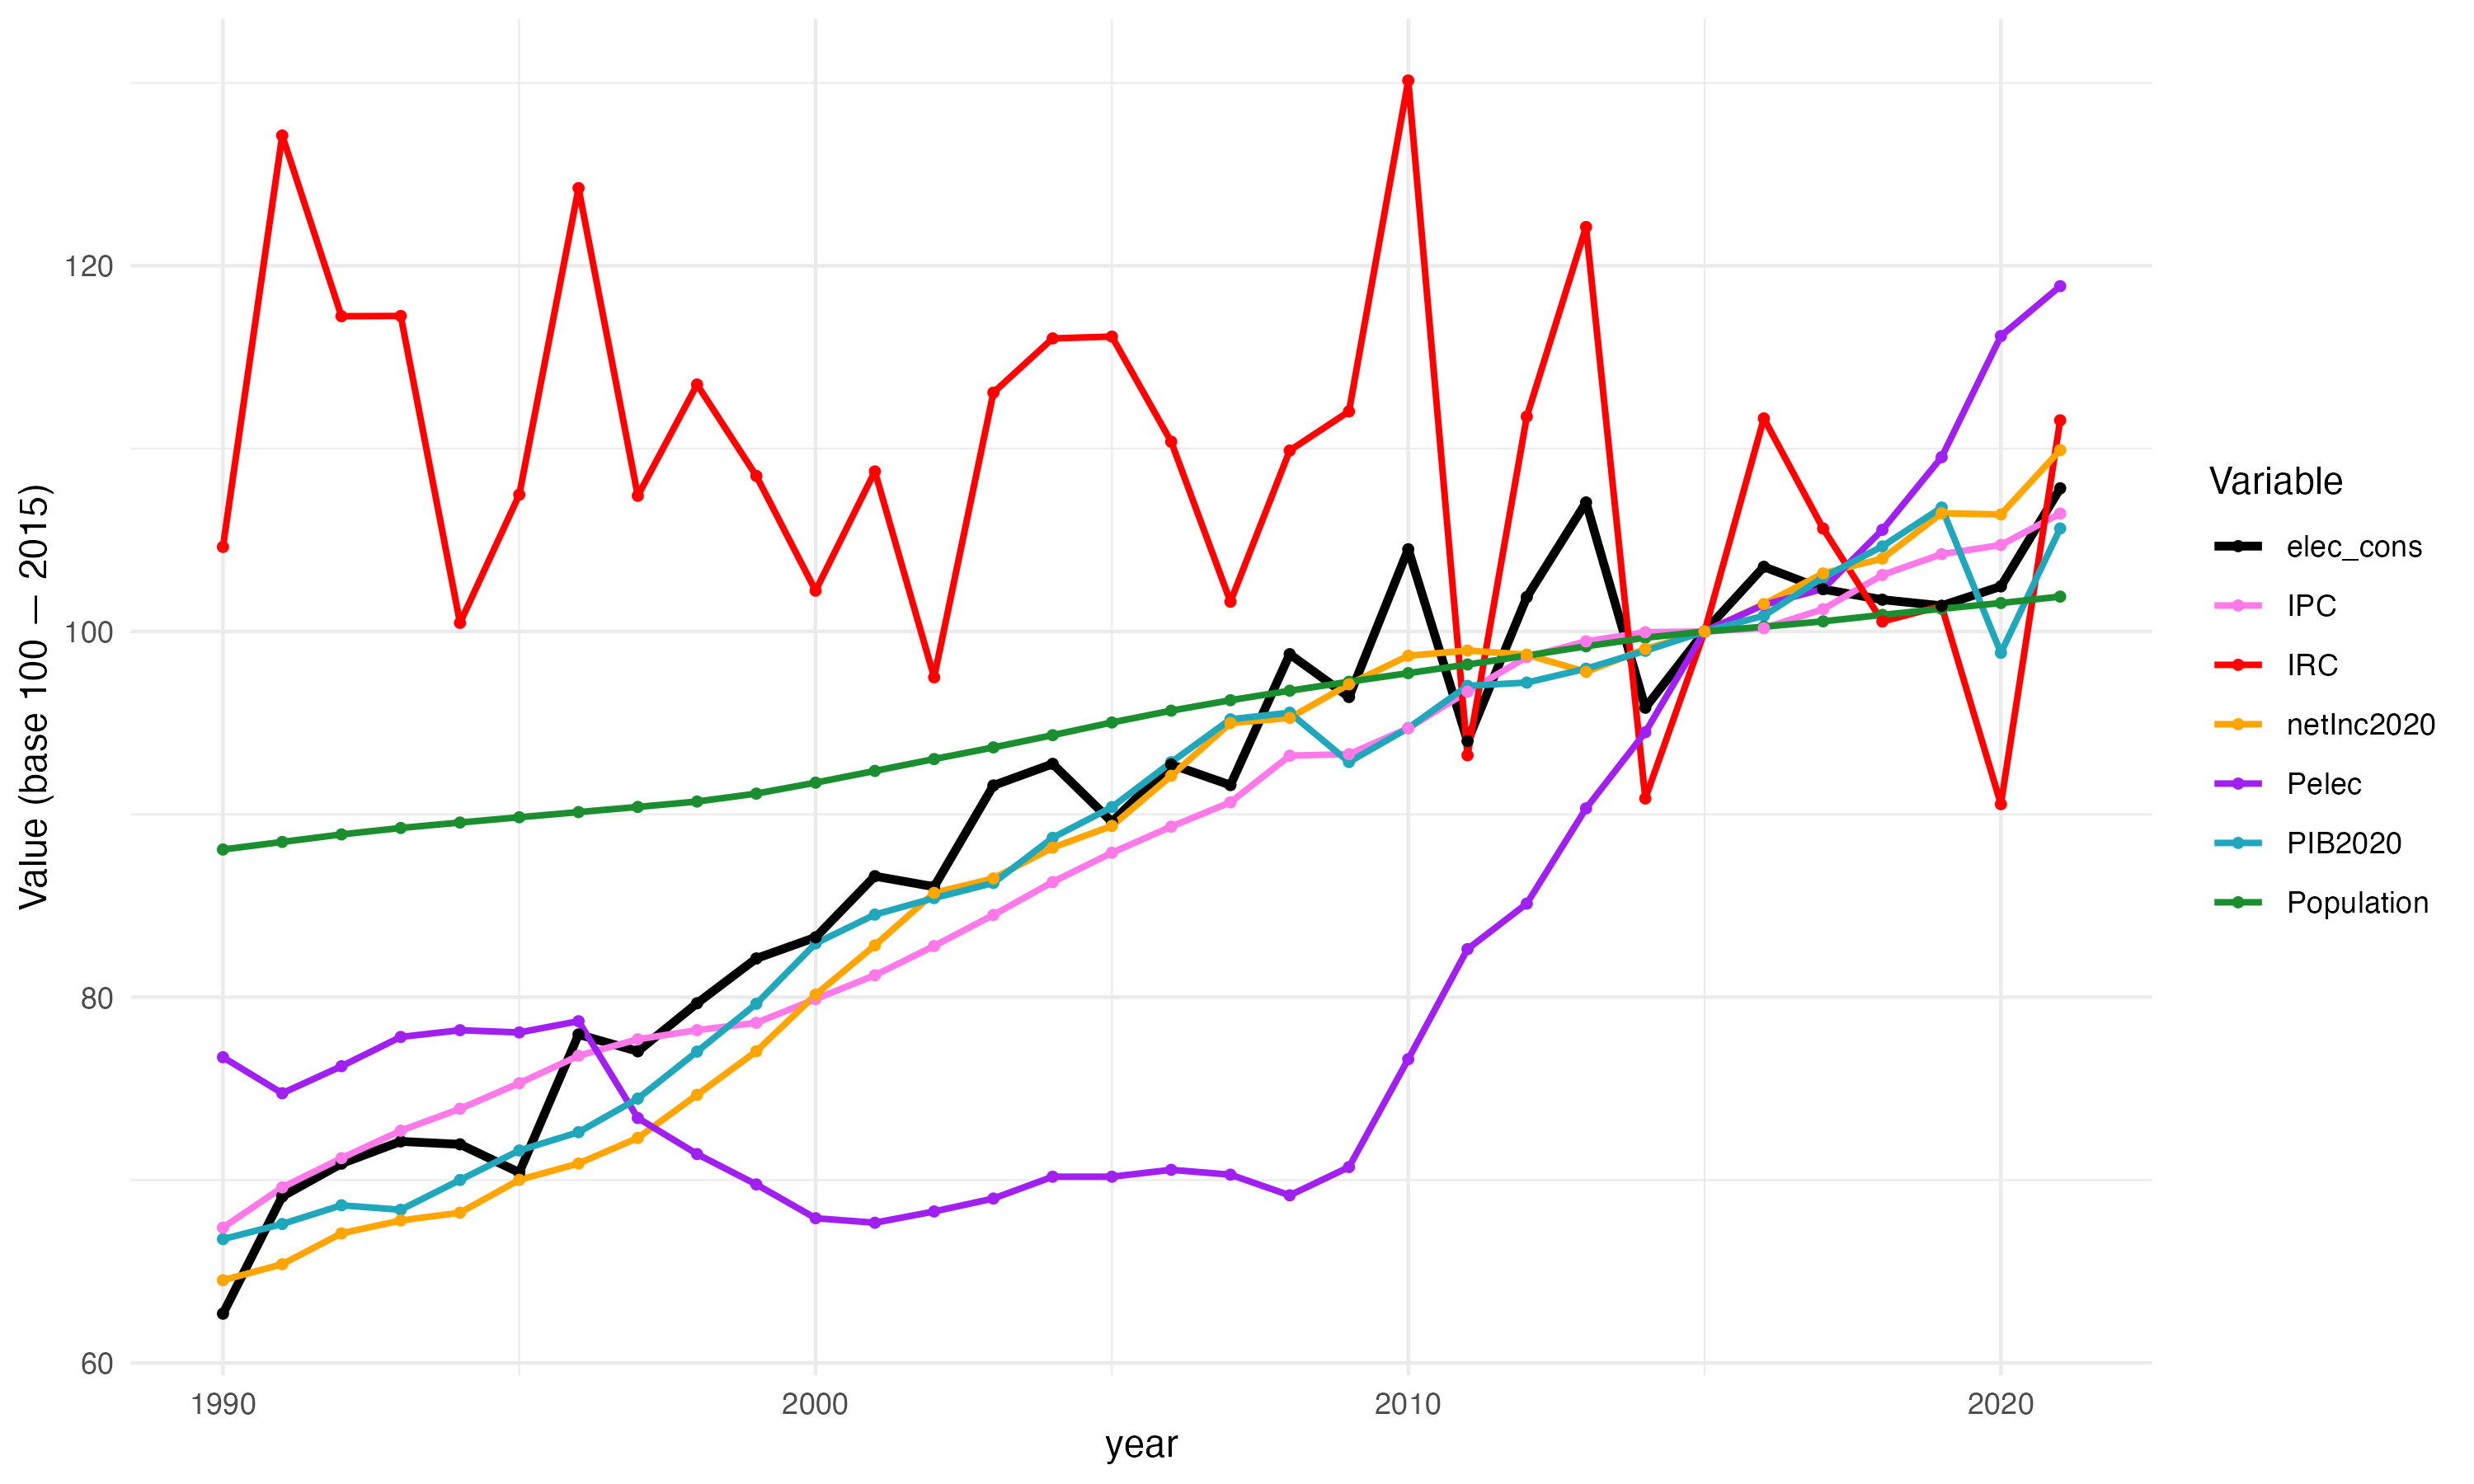
\includegraphics[width=0.5\textwidth]{Images/data_base100_2015.jpeg}
      \caption{Time variation in our data, expressed in base 100 (2015). In black the electricty consumption. In light blue and orange, respectively the GDP and the net disposable income, in euros 2020. In pink, the inflation through CPI, in green the population size. In red the climate index, and eventually in purple the electricity price.}
    \label{var}
  \end{figure}

From figure \ref{var}, we realize how close the GDP and the net disposable income are, only clearly diverging in trend in 2008 and 2020, which we can identify as the 2008 financial crisis and the Covid-19 crisis. Let us note that from 2008, the growth rate of electricity price becomes greather than inflation.

It seems of great matter to take into account the climate variable into our regression model, considering how electricity consumption peaks in cold winters. Eventually, we guess a correlation between the trend decline in the growth rate of electricity consumption and the burst in the price of electricity since 2009. It is likely that this sharp increase is a consequence of the 2008 energy crisis (which might be explained as the interaction of a strong positive demand shock and the ongoing financial crisis, maybe combined with the conventional oil peak that occurred around 2005-2008 \cite{delannoy2021peak}). Some market effect could also be considered, as competitive electricity markets are at play in the UE since 2007, and the treaty of Lisbon entered into force in 2009.

\begin{figure}[h]
    \centering
    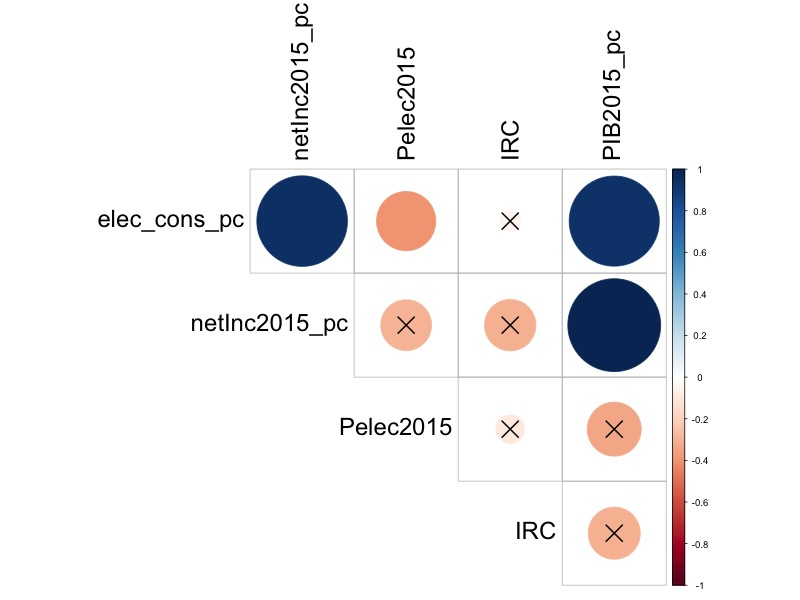
\includegraphics[width=0.5\textwidth, trim={0 0 0 5pt}, clip]{Images/correlation_matrix.jpeg}
        \caption{A correlation matrix of some data of interest. A cross indicate a p-value higher than 0.05 (no significant correlation).}
    \label{corr_mat}
  \end{figure}

The figure \ref{corr_mat} informs us of the correlation between some variable of interests, namely the electricty consumption per capita (\texttt{elec\_conc\_pc}), the net income per capita (\texttt{netInc2015\_pc}) and GDP per capita (\texttt{PIB2015\_pc}), the electricity price (\texttt{Pelec2015}) and the climate index (\texttt{IRC}). It reinforces our idea that the electricity consumption is negatively correlated with its price, and on the contrary that net disposable income and GDP are strongly correlated and might be used interchangeably.


\subsection{OLS Regression: a kind reminder}
For $n$ observations and $k$ variables, we use the following linear regression model:
\begin{align*}
    \boldsymbol{Y} & = \boldsymbol{X} \boldsymbol{\beta} + \boldsymbol{\varepsilon} \\
    \begin{bmatrix} 
        y_1 \\ y_2 \\ \vdots \\ y_n 
        \end{bmatrix} & = \begin{bmatrix}
        x_{11} & x_{12} & \cdots & x_{1k} \\ 
        x_{21} & x_{22} & \cdots & x_{2k} \\ 
        \vdots & \vdots & \ddots & \vdots \\ 
        x_{n1} & x_{n2} & \cdots & x_{nk} 
        \end{bmatrix} \begin{bmatrix}
        \beta_1 \\ \beta_2 \\ \vdots \\ \beta_k 
        \end{bmatrix} + \begin{bmatrix} 
        \varepsilon_1 \\ \varepsilon_2 \\ \vdots \\ \varepsilon_n \end{bmatrix}
\end{align*}

Ordinary Least Square (OLS) method is used to estimate the coefficients $\boldsymbol{\beta}$. It holds over the following hypothesis:
\begin{enumerate}
    \item More observations than explanatory variables.
    \item Absence of multicollinearity (mandatory assumption).
    \item Explanatory variables rely on data and the error term is random.
    \item The expected value of the error term is zero.
    \item Errors are not autocorrelated.
    \item Errors are homoscedastic.
    \item The error terms follow a normal distribution (for good properties).
\end{enumerate}

If the hypotheses 4, 5 and 6 are verified, the error term is a white noise. 

The $R^2$ coefficient is used to evaluate the goodness of fit of the model. It measures the proportion of the variance in the dependent variable that is predictable from the independent variables. The adjusted $R^2$ is used to compare the goodness of fit of models with different numbers of variables.

Confidence interval for $\beta_j \in \{\beta_1, \beta_2, \ldots, \beta_k\}$ is given by a Student's t-distribution with $n - k - 1$ degrees of freedom.

\subsection{First models}
The regression equation \eqref{eq:reg} is a model of electricity consumption seeking to explain the logarithm of per capita electricity consumption by the logarithm of income per capita in constant currency and the logarithm of the price of electricity in constant currency. 

\begin{equation} \label{eq:reg}
\ln{\frac{c_{elec_i}}{pop_i}} = \alpha + \beta_1 \ln{\frac{{netInc_i}}{pop_i}} + \beta_2 \ln{\frac{price_{elec_i}}{IPC_i}} + \beta_3 IRC_i + \varepsilon_i
\end{equation}

From an economic point of view, the consumption of a good could be explained by an income effect and a price effect, to which other effects may be added if necessary. Here, we add the Climate Rigor Index (\textit{Indice de Rigueur Climatique}, IRC) to control for climate variation (\textit{e.g.} a colder winter increases electricity consumption).

$\beta_1$ and $\beta_2$ represent respectively the income elasticity and the price elasticity of electricity consumption, \textit{i.e.} the percentage change in electricity consumption in relation, respectively, to a percentage change in income and the percentage change in prices. 

The table \ref{regression_full_pc} could have shown predictable results, as the income elasticity is positive (the bigger the income the bigger the consumption) and the price elasticity is negative (the bigger the price the smaller the consumption) and low (because electricity is a necessity, the demand might be inelastic to prices). However, the latter is not well captured by the model: the price coefficient is not significant. We thus decide to add an interaction term between income and price to the model, as in equation \eqref{eq:good} (setting $y_i = \ln{\left(\frac{c_{elec_i}}{pop_i}\right)}$). 
\begin{align} \label{eq:good}
    &y_i = \alpha + \beta_1 \ln{\left(\frac{{netInc_i}}{pop_i}\right)} + \beta_2 \ln{\left(\frac{price_{elec_i}}{IPC_i}\right)} \notag \\
    &+ \beta_3 IRC_i + \beta_4 \ln{\left(\frac{{netInc_i}}{pop_i}\right)} \times \ln{\left(\frac{price_{elec_i}}{IPC_i}\right)} + \varepsilon_i
\end{align}
Let us see if the OLS assumptions hold. 

\subsubsection{Multicollinerarity}
The Variance Inflation Factor (VIF) of all variables but IRF was over $2000$, indicating huge multicollinearity. Because of the few variables and the small sample size we have, variable selection and regularization methods like LASSO or Elastic Net would not make any sense. In order to keep the interaction, we apply mean-centering to our variables of interests.
\begin{equation} \label{eq:mean-cent-operator}
    \begin{cases}
    \text{ln-Inc-pc} = \ln{\left(\frac{{netInc_i}}{pop_i}\right)} = X_1 & \Rightarrow {X}_1^{(MC)} = X_1 - \bar{X}_1\\
    \text{ln-price2015} = \ln{\left(\frac{price_{elec_i}}{IPC_i}\right)} = X_2 & \Rightarrow {X}_2^{(MC)} = X_2 - \bar{X}_2\\
    \end{cases}
\end{equation}

The regression therefore becomes: 
\begin{align} \label{eq:OLS-mean-cent}
    & y_i = \alpha + \beta_1 \left(\text{ln-Inc-pc}_i^{(MC)}\right) + \beta_2 \left(\text{ln-price2015}_i^{(MC)}\right) \notag \\
    & + \beta_3 IRC_i + \beta_4 \left(\text{ln-Inc-pc}_i^{(MC)} \times \text{ln-price2015}_i^{(MC)}\right) + \varepsilon_i
\end{align}
Using model \eqref{eq:OLS-mean-cent}, we don't face multicollinearity anymore: our VIF values for all variables stands between $1$ and $3$. The following tests are performed on this model.

\subsubsection{Normality of residuals}
It is known that the Kolmogorov-Smirnov test is less powerful for testing normality than the Shapiro-Wilk test or Anderson-Darling test. Because the Shapiro-Wilk does not work well with many identical values and the Jarque-Bera test is not efficient for small samples, we choose the Anderson-Darling test to see whether the error terms follow a normal distribution. The test provides a p-value of $0.2989$, so we do not reject the null-hypothesis that the residuals are normally distributed. Also, we performed a one sample t-test on the residuals to control for the null hypothesis that the mean of the residuals is zero, which is true.

\subsubsection{Homoscedasticity}
The White test can detect a wide range of forms of heteroskedasticity, but tends to falsely detect heteroscedasticity in small samples. The {Breusch-Pagan} test is designed to detect only linear forms of heteroskedasticity, and even though the Goldfeld–Quandt test is not very robust to specification errors, it performs better for small samples. Both Breusch-Pagan and Goldfeld–Quandt tests give a p-value over $0.7$, so we can admit that the residuals are homoscedastic.

\subsubsection{Autocorrelation}
Three tests can be used: the Durbin-Watson test is valid for nonstochastic regressors and allows to test the possibility of a first-order autoregressive model (e.g. AR(1)) for the regression errors. The Ljung-Box test, which requires the assumption of strict exogeneity, controls for higher order autocorrelation. 
The Breusch–Godfrey test is statistically more powerful than Durbin's h statistic and more general than the {Ljung-Box} test. It checks for serial correlation and requires the assumptions of stronger forms of predeterminedness and conditional homoscedasticity.

Performing the tests (see table \ref{autocorrelation_tests}) reveals that the model does not suffer from autocorrelation, the residuals are independent, even we looking at multiple lags.
\begin{table}[h]
    \centering
    \caption{Autocorrelation Test Results}
    \label{autocorrelation_tests}
    \begin{tabular}{lccc}
    \\[-1.8ex]\hline 
    \hline \\[-1.8ex] 
    Test & Statistic & DF & p-value \\
    \hline
    Durbin-Watson & 1.7639  & NA & 0.1066 \\
    Ljung-Box (lag=10) & 11.8304  & 10 & 0.2966 \\
    Breusch-Godfrey & 0.1482  & 1 & 0.7003 \\
    \hline
    \end{tabular}
\end{table}

\subsubsection{Results}
The model \eqref{eq:OLS-mean-cent} passed all the tests: it is well specified and can be interpreted. The table \ref{regression_good_linear} shows the results of the regression. The $R^2$ and adjusted $R^2$ are around 0.96, meaning that the model explains most of the variance in the dependent variable. The F-statistic is high with $p-value < 2.2e-16$, meaning that the model is statistically significant. 

\begin{table}[!htbp] \centering 
    \caption{Regression analysis results from model \eqref{eq:reg}.} 
    \label{regression_full_pc} 
  \begin{tabular}{@{\extracolsep{0pt}}lc} 
  \\[-1.8ex]\hline 
  \hline \\[-1.8ex] 
   & \multicolumn{1}{c}{\textit{Dependent variable:}} \\ 
  \cline{2-2} 
  \\[-1.8ex] & log(elec\_cons\_pc) \\ 
  \hline \\[-1.8ex] 
   log(netInc2015\_pc) & 0.859$^{***}$ \\ 
    & (0.044) \\ 
    & \\ 
   log(Pelec2015) & $-$0.057 \\ 
    & (0.039) \\ 
    & \\ 
   IRC & 0.269$^{***}$ \\ 
    & (0.057) \\ 
    & \\ 
   Constant & $-$9.563$^{***}$ \\ 
    & (0.212) \\ 
    & \\ 
  \hline \\[-1.8ex] 
  Observations & 32 \\ 
  R$^{2}$ & 0.944 \\ 
  Adjusted R$^{2}$ & 0.938 \\ 
  Residual Std. Error & \makecell{0.026 \\ (df = 28)} \\  % Multi-line with makecell
    F Statistic & \makecell{157.060$^{***}$ \\ (df = 3; 28)} \\  % Multi-line with makecell 
  \hline 
  \hline \\[-1.8ex] 
  \textit{Note:}  & \multicolumn{1}{r}{$^{*}$p$<$0.05; $^{**}$p$<$0.01; $^{***}$p$<$0.001} \\ 
  \end{tabular} 
\end{table} 

\begin{table}[!htbp] \centering 
    \caption{Regression analysis results from model \eqref{eq:OLS-mean-cent}.} 
    \label{regression_good_linear} 
    \begin{tabular}{@{\extracolsep{0pt}}lc} 
        \\[-1.8ex]\hline 
        \hline \\[-1.8ex] 
         & \multicolumn{1}{c}{\textit{Dependent var.:}} \\ 
        \cline{2-2} 
        \\[-1.8ex] & log(elec\_cons\_pc) \\ 
        \hline \\[-1.8ex] 
         ln\_Inc\_pc\_MC & 0.720$^{***}$ \\ 
          & (0.055) \\ 
          & \\ 
         ln\_price2015\_MC & $-$0.104$^{**}$ \\ 
          & (0.036) \\ 
          & \\ 
         IRC & 0.293$^{***}$ \\ 
          & (0.049) \\ 
          & \\ 
         ln\_Inc\_pc\_MC:ln\_price2015\_MC & 1.348$^{**}$ \\ 
          & (0.387) \\ 
          & \\ 
         Constant & $-$13.295$^{***}$ \\ 
          & (0.049) \\ 
          & \\ 
        \hline \\[-1.8ex] 
        Observations & 32 \\ 
        R$^{2}$ & 0.961 \\ 
        Adjusted R$^{2}$ & 0.956 \\ 
        Residual Std. Error & \makecell{0.022 \\ (df = 27)} \\ 
        F Statistic & \makecell{167.504$^{***}$ \\ (df = 4; 27)} \\ 
        \hline 
        \hline \\[-1.8ex] 
        \textit{Note:} $^{*}$p$<$0.05; $^{**}$p$<$0.01; $^{***}$p$<$0.001  & \multicolumn{1}{r}{} \\ 
    \end{tabular} 
\end{table} 
        

In the model $y_i = \alpha + \beta_1 X_{1_i} + \beta_2 X_{2_i} + \beta_3 X_{3_i} + \beta_4  X_{1_i} X_{2_i} + \varepsilon_i$, the elasticity of $X_j$ on $y$ is given by $\frac{\partial y}{\partial X_j}$. Therefore, the new net income per capita and price elasticities of electricity consumption are defined as: 
\begin{equation} \label{eq:elast}
    \begin{cases}
    \text{Income elast.:} & \beta_{Inc} = \beta_1 + \beta_4 \text{ln-price2015}^{(MC)}\\
    \text{Price elast.:} & \beta_{price} =\beta_2 + \beta_4 \text{ln-Inc-pc}^{(MC)} \\    
    \end{cases}
\end{equation}

Because of the mean-centering, $\beta_1$ and $\beta_2$ capture the baseline effect of a variable at its sample mean while $\beta_4$ represents how the effect of price depends on income in relation to the average income per capita level.

The new elasticites expression given equation \eqref{eq:elast} are precious to understand the regression coefficients given table \ref{regression_good_linear}, as it can be shown that for any observation $i$, $\beta_{Inc} > \beta_1 = 0.720$ and $\beta_{price} < \beta_2 = -0.104$ (because $\forall i, \text{ln-price2015}^{(MC)}_i > 0$ and $\text{ln-Inc-pc}^{(MC)}_i < 0$). 

Thus, classic microeconometric results are found as there is a negative price elasticity and a positive income elasticity of electricity consumption. The more expensive electricity is, the less people will consume it, and the richer they are, the more they will consume. We should nonetheless highlight the fact that the upper bound of $\beta_{price}$, $\beta_2$, is close to an inelasticity threshold: because electricity is a necessary good, the price effect is lower than the income effect, due to the households' non-compressible electricity consumption. $\beta_3$ value also leads to an obvious result: the colder a winter is, the more electricity is consumed.

The interaction term is positive, meaning that the price elasticity of electricity consumption increases with income. If income increases, the price effect becomes less negative: this could be explained by the fact that after a certain level of income, households are less sensitive to price changes. On the other way around, if electricity prices rise, income has a stronger positive effect on consumption.

\subsection{Structural break}
We previously mentioned how 2008 seemed to be a turning point in the electricity price trend and how it could have affected the electricity consumption trend. Let us use statistical techniques to detect whether or not this break matter. 

Bai and Perron (1998, 2003) provided a theoretical framework and computational algorithms to estimate and test for multiple structural changes at unknown dates in linear regression models, where the regressors are non-trending or regime-wise stationary \cite{bai1998estimating, bai2003computation}. 

The Bai-Perron multiple break test \cite{bai1998estimating} identifies $m$ breakpoints as $t_1^, t_2^, \dots, t_m^*$ by minimizing the sum of squared residuals (SSR) across different segments. 

$$\sum_{j=1}^{m+1} SSR(y_{t_{j-1}+1:t_j})$$

where $t_0 = 1$ and $t_{m+1} = T$. 

First, by computing the sequential $\sup F$ tests of $l$ versus $l+1$ for $l \in \{1, \dots, m\}$ with each corresponding null hypothesis of maximum number of break is $l$ and alternative hypothesis is $l+1$, we can identify the number of breakpoints. Then, knowing the number of breakpoints, we can compute a structural change model and split the dataset into separate regimes. 

Therefore, Bai-Perron Test is particularly useful as it can found multiple unkown breaks while handling potential heteroskedasticity and serial correlation.

On the contrary, the Chow test \cite{chow1960tests} is used to test whether a structural break occurs at a specific, pre-determined date, assuming OLS properties. To perform a Chow test, we need to split the sample at the known break date into two subsamples. Then, we estimate the regression separately for both subsamples and for the entire dataset (without a break). To test whether the coefficients before and after the break are significantly different, we use the following F-statistics:
$$F = \frac{(SSR_r - (SSR_1 + SSR_2)) / k}{(SSR_1 + SSR_2) / (n_1 + n_2 - 2k)}$$

where $SSR_r$ is Sum of squared residuals for the full model, $SSR_1, SSR_2$ the one for the "before" and "after" models, $k$ the number of parameters in the model and $n_1, n_2$ the number of observations in each segment. \\

Justify two breaks. 
Add graphs. 
Talk about regression on the last subset, the lack of significance because of the too small sample size. 

Then use dummies to do a regression and capture the breaks (add one for COVID). Then forecasting.

\subsection{A change of strategy}
Lags? Why would the model be better with lags: does past prices or past income affects current consumption? \\

Why would the model be better with autoregression: does previous consumption influence current consumption? \\

First: Stationarity: Check whether your variables are stationary using Augmented Dickey-Fuller (ADF) tests. If they are not, you should difference them. \\

3. Consider Economic Cycles and Policy Shocks
    \begin{itemize}
        \item Economic activity affects electricity demand non-linearly. Add:
        \begin{itemize}
            \item A squared GDP term $(\ln{\frac{{PIB}}{pop}}^2)$ to check for diminishing returns.
            \item A crisis dummy for 2008-2009 (financial crisis) and 2020 (COVID-19).
        \end{itemize}
        \item The IRC coefficient is positive and significant, meaning harsher winters increase electricity demand.
        \item Use interaction effects:
        \begin{itemize}
            \item $\text{IRC} \times \ln{\frac{PIB}{pop}}$ to check if income affects sensitivity to climate.
            \item Do the same with income and sensitivity to price.
        \end{itemize}
    \end{itemize}


(to check if income affects sensitivity to climate). Do the same with income and sensitivity to price. \\


\section{Results}

\section{Limits}
Disaggregate income by quintile to highlight the impact of income inequality on electricity consumption. \\

Should the electricity price be considered as an endogenous variable from the moment energy markets were liberalized? When prices are no longer set by public authorities, its variation could indeed be explained by the demand for electricity: the use of instrumental variables would then be necessary to avoid endogeneity bias.

\section{Matériels et méthodes}
\label{Méthodes et Matériel}

\begin{figure}[h]
  \centering
    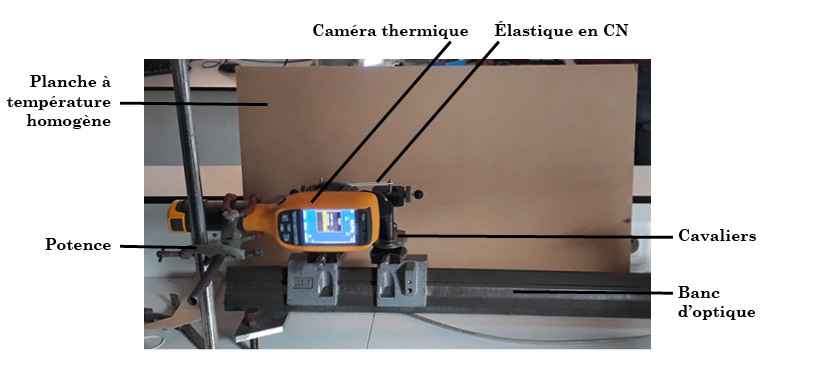
\includegraphics[width=0.54\textwidth]{Images/dispositif_legende.png}
     \vspace*{-0.8cm}
    \caption{\small{Photographie légendée du dispositif expérimental sur lequel nous avons effectué toutes nos expériences. La planche placée derrière le banc permet d'uniformiser le champ de température afin que seules les variations de température des élastiques soient enregistrées.}}
        \label{dispositifexp}
    \vspace*{-0.4 cm}
\end{figure}









\section{Résultats et discussions}
\label{results}

\section{À propos du prototype}

%etc...
\section{Conclusion}
% pour créer un nouveau document en "XXX.tex" dans le fichier "sections" et ajouter dans le "main.tex" un input.
%-------------------------------Bibliographie-----------------------------------

\vspace{-0.32cm}
\nocite{*}
\bibliographystyle{unsrt}
\bibliography{biblio.bib}   % Voir le fichier "biblio.tex"
\addcontentsline{toc}{section}{Bibliographie}

\section{Documents complémentaires}

\end{document}
%------------------------------Fin du document----------------------------------